\documentclass{article}

\usepackage[
        bibencoding=utf8, 
        style=alphabetic
    ]{biblatex}

\bibliography{bibliography}

\usepackage{arxiv}

\usepackage[utf8]{inputenc} % allow utf-8 input
\usepackage[T1]{fontenc}    % use 8-bit T1 fonts
\usepackage{hyperref}       % hyperlinks
\usepackage{url}            % simple URL typesetting
\usepackage{booktabs}       % professional-quality tables
\usepackage{amsfonts}       % blackboard math symbols
\usepackage{nicefrac}       % compact symbols for 1/2, etc.
\usepackage{microtype}      % microtypography
\usepackage{lipsum}		% Can be removed after putting your text content
\usepackage{graphicx}


\title{\emph{ApakoHa}: an automated tool using dynamic taint analysis for android security focusing on sensitive data}

%\date{September 9, 1985}	% Here you can change the date presented in the paper title
%\date{} 					% Or removing it

\author{
  Yiwei Yang, Longwen Zhang, Kaiyuan Xu, Zhe Ye \\
  Schools of Information and Science Technology\\
  ShanghaiTech University\\
  Shanghai, SH 201210 \\
  \texttt{yangyw,zhanglw2,xuky,yezhe@shanghaitech.edu.cn} \\
}


\begin{document}
\maketitle

\begin{abstract}
  Privacy protection on android phones is a widely discussed topic nowadays. As the main leaking source, many tools analyzing information flow statically and dynamically. Integrating dynamic taint analysis in the development process enables early detection of potential privacy leakage, which reduces the cost of fixing them.
  In this paper, we present \emph{ApakoHa}, a dynamic taint analysis tool for Android apps that interleaves bug fixing and code development in the VS-code integrated development environment. 
  \emph{ApakoHa} is based on the novel framework of TaintART that makes full use of android ART runtime to get information flow, and computes the more complex results and optimizes the bytecode through soot\ref{fig:FlowDroid1}. incrementally later using static analyzing tools. Unlike traditional batch-style static-analysis tools, \emph{ApakoHa} causes minimal disruption to the developer’s workflow. This video
demo showcases the main features of \emph{ApakoHa}: http://bilibili.com/video/av82222945/

\end{abstract}


% keywords can be removed
\keywords{DTA \and Android privacy \and automated tool \and operating system}


\section{Introduction}
Android security has attracted much research attention from both academy 
            and industry recently. Dynamic Taint Analysis(DTA) is a classic analysis to detect
             information flow problems and it has been widely adopted to detect private
             data leaks in Android applications. In this project, \emph{ApakoHa} will automate the
             process of taint analysis and provide more detailed information about the dataflow and ICFG on the source code. Thus providing a way for Maple IR to continue to compile.

First, in terms of the performance of the DTA, we refer to the TaintART techniques to utilize the 
            compiler and the register allocation of android ART Runtime. Then, a taint propagation 
            framework is proposed and the correctness of the taint propagation analysis is proved by 
            their paper. After \emph{ApakoHa} obtains the information flow and what kind of method the information is leaking, we try to make highlight the code on VS-Code front end,
            Finally, in the backend, the function name and the taint source will be input to soot, a java static analyzing tool to output ICFG and optimize the code automatically  by adopting the methods of eliminating, replacing and moving.

\emph{ApakoHa} is actually adopting the method of combing the advantages of dynamic and static taint analysis techniques. Through static analysis can sort out the general idea, through dynamic analysis can get the actual execution process of the program. Both of them can help each other to realize the deep penetration test of the responsible app. The pros and cons of the state of art are listed as follows:

\begin{table}
  \caption{The comparison of the state of the art android taint analysis}
   \centering
   \begin{tabular}{llll}
     \toprule
     Type     & Representative works &     & Features \\
     \midrule
           & In-component propagation analysis &LeakMiner/CHEX  & Incrementally add callback function \\
            &                                   &                 &  Implementing the Android semantic equivalent model     \\
            &                                   &                 &  Add processing callback function Virtual access point    \\
      
           &  & &     \\
      Static & Inter-component propagation analysis &Klieber  &Match with custom inference rules    \\
           &  &Heros/DroidSafe & Transform data flow analysis to improve accuracy     \\
           &  & &     \\
           &  Component and library & FlowDroid& Manual analysis and Implementation \\
           & function propagation analysis & &    Automatic derivation with FlowDroid   \\
           &  & &     \\
     Dynamic & Multi level propagation analysis&TaintDroid & Address multiple levels of communication strategy      \\
           &   & Appsplaygroud...   & Optimization or application extension  \\
     \bottomrule
   \end{tabular}
   \label{tab:table1}
 \end{table}


\section{Related workflow}

\subsection{Taintdroid}
TaintDroid \ref{sec:TaintDroid} is a system-wide taint tracking system based on Android 4.2+. It aims to minimize runtime overhead that is the amount of additional instructions needed for the implementation of tracking mechanism and, also to monitor the system for sensitive information leakage.


\begin{figure}[ht]
  \centering
  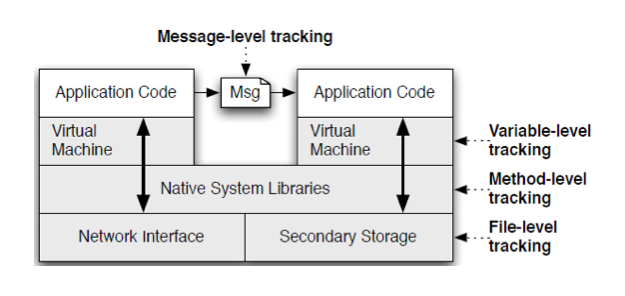
\includegraphics[scale=0.6]{TaintDroid.png}
  \caption{TaintDroid Multi-level tracking.}
  \label{fig:TaintDroid}
\end{figure}

As shown in Figure \ref{fig:TaintDroid}, the system tracks information at multiple levels. The variable-level tracking means the information flow among memory like stack register and heap object. The method-level tracking means the whenever a method returns, the return value if any should properly propagate to the caller method. The file-level tracking means that the system store taint tag on file system permanently. The message-level tracking means the information flow between processes. An Android application typically uses the broadcast receiver and intent to communicate with each other
.

TaintDroid uses technique call adjacent memory storage for the taint storage. This means taint tag locates next to the memory which the tag is associated with. In theory, this implementation should double both the total memory and the address of object. This eases the calculation of the address of the taint tag.


The taint tag used by TaintDroid is bit-wise, meaning each bit of the allocated memory represents the absence or presence of certain type information. The taint tag is stored in a 32-bit integer. As a result, only 32 types of information can be distinguished. There are several modifications made by TiantDroid developers for the accommodation of taint tag.

1. Stack. Next to each virtual register which is just a 4-byte memory, an additional 4-byte memory is allocated so that during the execution of a method, the taint tag can be stored locally for the method.

2. Calling convention. When a method is invoked or returned, a modified calling convention is used to accommodate the taint tag for the return result.

3. Parcel. This change allows taint tag travel through binder which essentially the inter-process communication procedure.

4. File system. TaintDroid extends the Linux file system so that the metadata on INode can store the taint tags. If such way, a file which receives sensitive information can be marked accordingly. In such way, taint tag can be stored permanently.

With the propagation rules, taint tag can travel through the application and system and when
the information flows to the predefined method or sink, the situation is reported through a special channel and revealed by a front application. For example, a binary operation like addition which takes in virtual register A and B and output to virtual register C. The resulted taint tag of register C should the union of taint tags from register A and B. The union operation in TaintDroid is used as binary "OR" operation. The Table 1 comes from TaintDroid and shows the propagation rules.

\begin{figure}[ht]
  \centering
  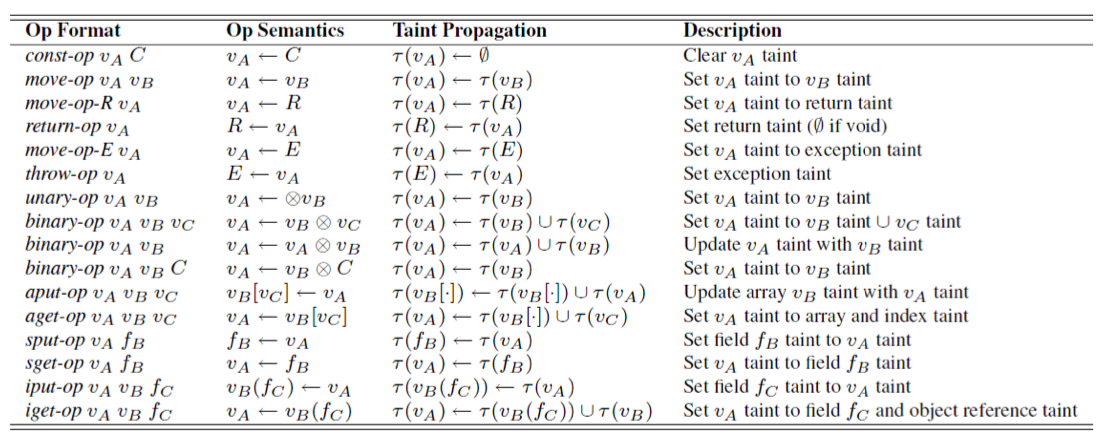
\includegraphics[scale=0.4]{TaintDroid2.png}
  \caption{TaintDroid Propagation Rules.}
  \label{fig:TaintDroid}
\end{figure}

TaintDroid is strong for the runtime efficiency. The statistic shows only 14\% runtime overhead occurring during testing. The drawback, however, is that the system is based on Android version 4.2 which is outdated compared today's version 7.0. TaintDroid cannot distinguish files but only label all files under one type of information.


\subsection{Cheetah}
Despite the demonstrated usefulness of DTA in mobile privacy security, poor performance attained by prototypes is a big problem. A novel optimization methodology for taint tracking based on just-in-time static analysis taht discovers and reports the most relevant results to the developer fast is presented. Cheetah\ref{sec:TaintDroid} is a JIT taint analysis for Android applications applying this theory. It enables easy transformation of a distributive dataflow analysis to its correstponding JIT with minimal changes to its fransfer functions. A JIT analysis computes the same dataflow propagations as its base analysis, but it delays some propagations in favor of others by pausing and resuming them later at trigger $stmt$, and each of them is assorciated with a priority that determines the layer at which the JIT analysis resumes its computation.

However, their work is not compatible with android development for from android 7.0 AoT take the place of JIT.
\subsection{Inspeckage}
Inspection is an Xposed module for dynamic analysis of Android apps. Inspection package summarizes many common functions of dynamic analysis and builds a web server. The whole analysis operation can be carried out in a friendly interface environment.

\begin{figure}[ht]
  \centering
  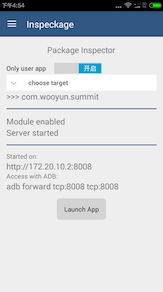
\includegraphics[scale=0.6]{inspeckage1.png}
  \caption{Inspeckage analyzing background.}
  \label{fig:inspeckage1}
\end{figure}

\begin{figure}[ht]
  \centering
  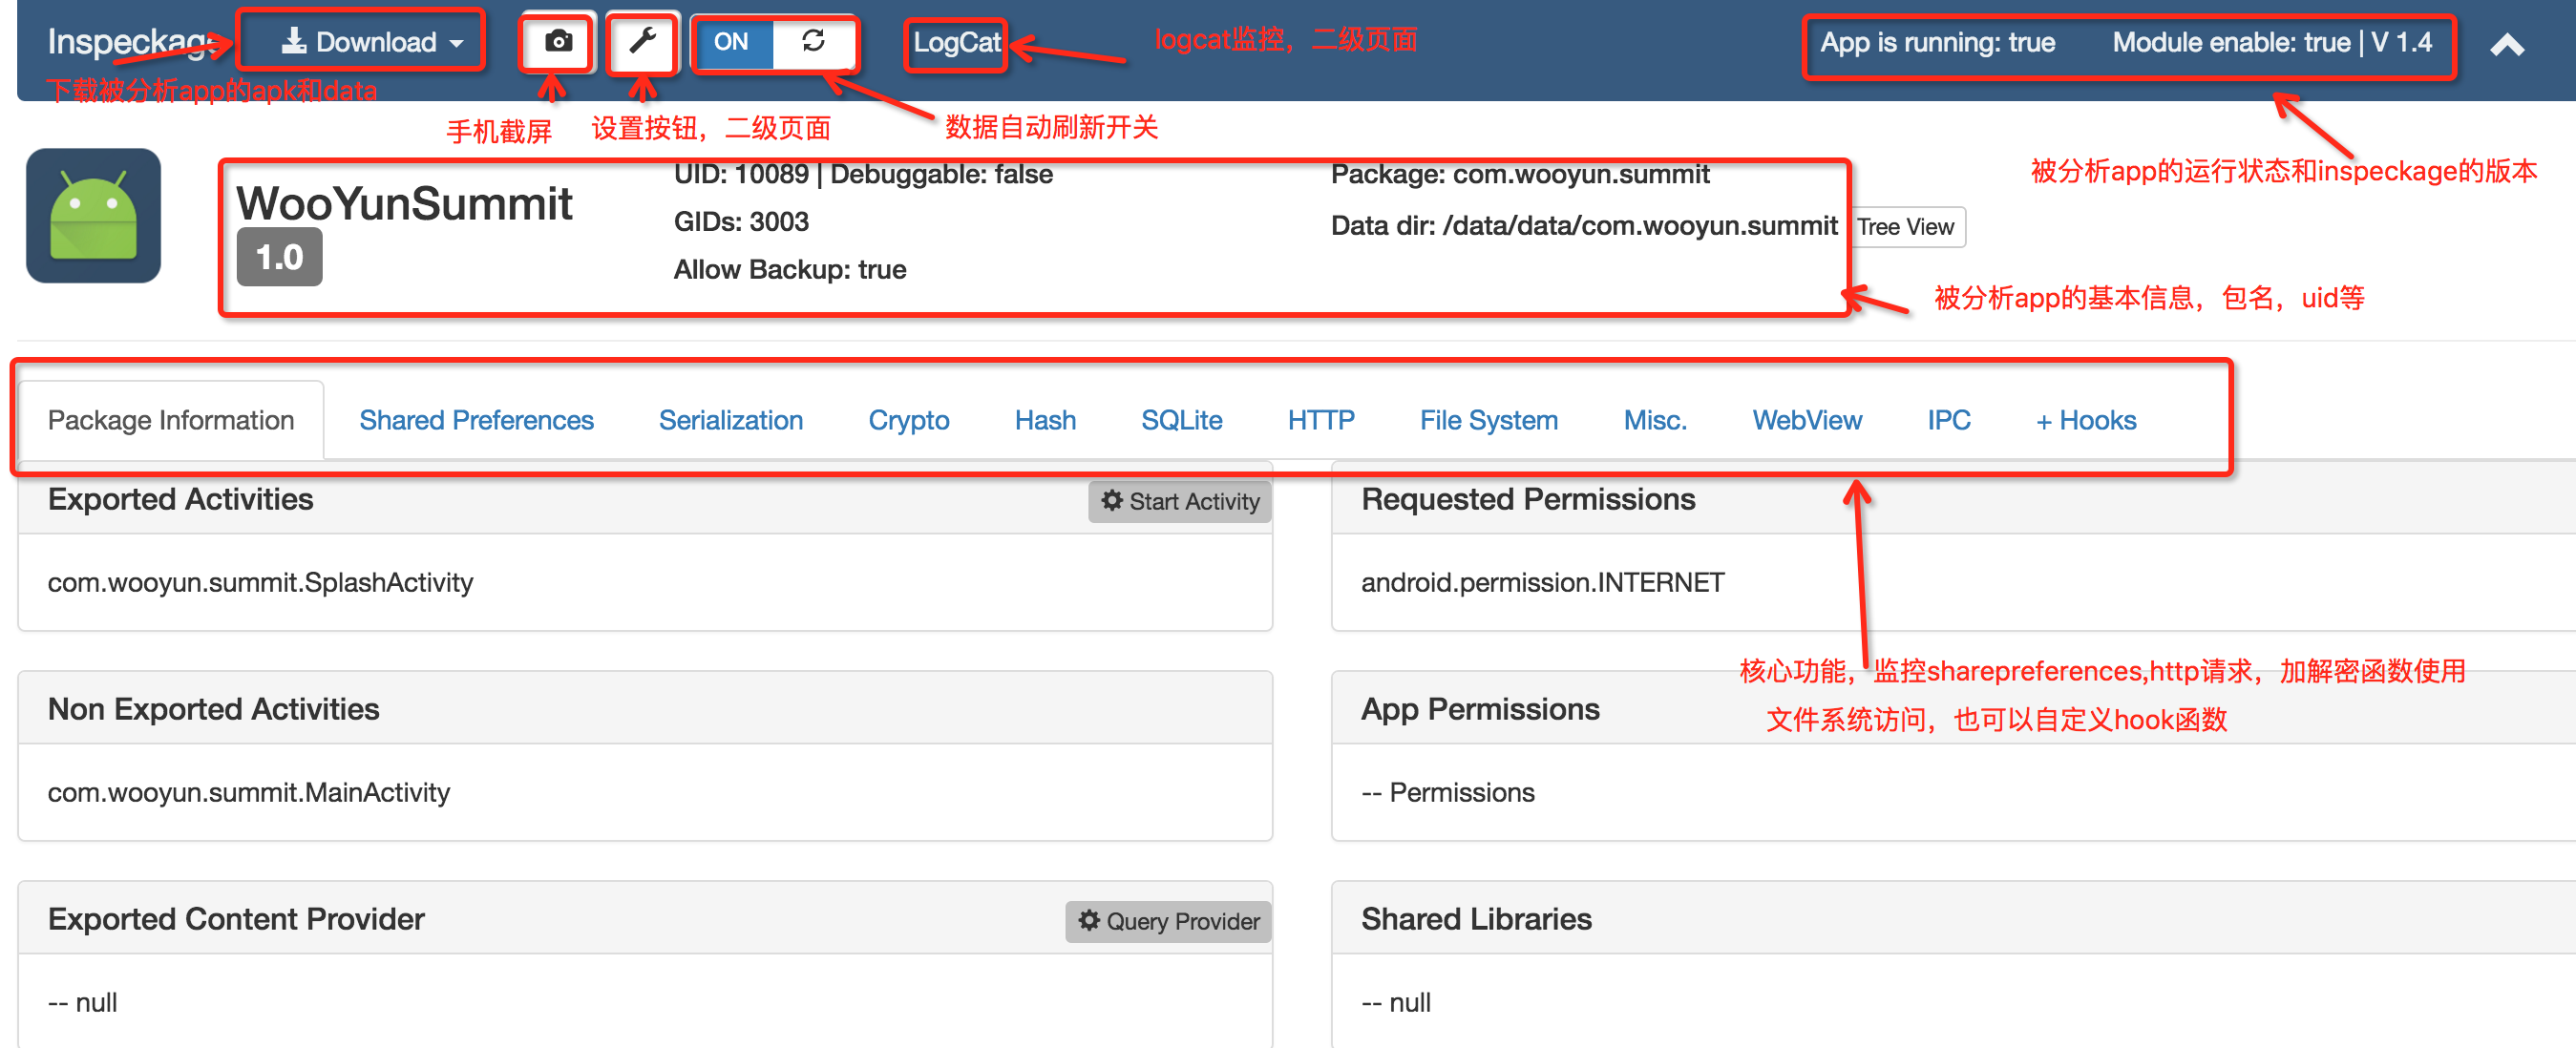
\includegraphics[scale=0.1]{inspeckage2.png}
  \caption{Inspeckage webserver.}
  \label{fig:inspeckage1}
\end{figure}

In theory, it can get all the information by add hooks, but it requires Xposed, which is depreacated since android 7.0.

\section{Theory Principles}
In this part, we'll introduce how the dynamic taint analysis work in tracking the private information and how we find the ICFG graph for those who have possibility to leak information in dynamic runtime which may save a lot of time analyzing non-triggered leakage situation.
\subsection{Principles of finding Information flow in DTA}
\begin{figure}[ht]
  \centering
  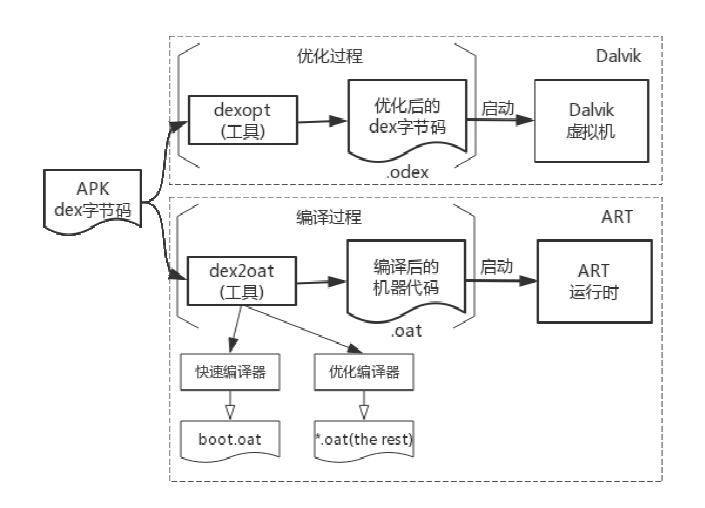
\includegraphics[scale=0.3]{TaintART1.png}
  \caption{TaintART ART runtime.}
  \label{fig:TaintART1}
\end{figure}
The main difference between DTA and STA is that DTA has to deal with the runtime. Somtimes hardware support is required. But in android, all the register allocation is based on ART runtime. 



For DTA, the sensitive data to be tracked is called taint source, and the tag added to track sensitive data is called taint tag. When sensitive data is copied or moved to another new location, or data is cleared, its tag will also be copied, moved or cleared, which is called taint logic In taint logic, the status of taint tags that track sensitive data will be stored in taint tag storage. DTA will track the tainted sensitive information and detect whether it is sent out of the system through certain functions, which are called taint sink.

\subsubsection{Runtime support}
The feature of TaintART is that it uses CPU register to store the taint tags. The taint tag is either 1 or 2 bits wide and represents the taint status of other processor registers. During the compilation, the program reserves register 5 and treats it as storage. The register 12 is used for taint propagation.


\subsubsection{Taint Source}
\begin{figure}[ht]
  \centering
  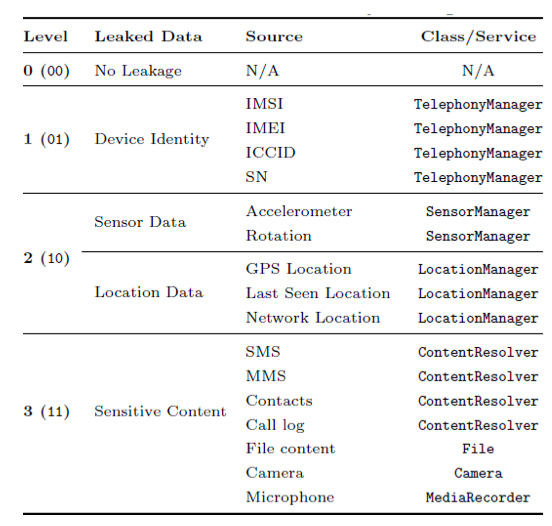
\includegraphics[scale=0.3]{TaintART2.png}
  \caption{TaintART Taint Source.}
  \label{fig:TaintART2}
\end{figure}


\subsubsection{Taint Propogation}
The propagation rules of TaintART shares some similarities with the one from TaintDroid \ref{fig:TaintDroid}. The major difference is TaintART’s rule focus on the instruction at compilation level. HInstruction is a class used by Android for the representation of each Dalvik instruction. The TaintART have rules for every HInstruction so that the resulted binary code can achieve taint propagation as desired. The second major difference is that the unlike binary or operation used by TaintDroid, the TaintART uses a special information merging operation. Take 2-bit wide storage for example. Suppose a taint tag of 0x01 needs to be merged with a taint tag of 0x010, the result would be 0x10. This is because the TaintART uses a level design. When a low-level taint tag encounters a higher-level taint tag, the result would simply be the higher one. The choice is made due to the privacy and runtime efficiency focus.
\begin{figure}[ht]
  \centering
  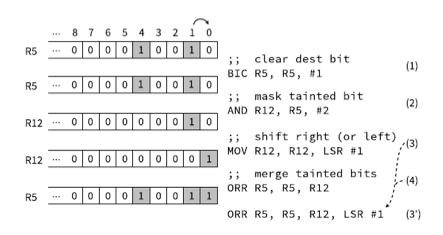
\includegraphics[scale=0.4]{TaintART3.png}
  \caption{TaintART Taint Propogation.}
  \label{fig:TaintART3}
\end{figure}

Figure \ref{fig:TaintART3} comes from TaintART and shows the operations done for the instruction "MOV R0, R1". The initial taint status represented by R5 is that register 1 and 4 are tainted. The result of MOV operation should leave register 0 tainted. The instruction \#1 masks bit on index 1 which represents the taint tag for register 1 and store the value into temporary register 12 in Instruction \#2. The instruction \#3 shifts the bit to the appropriate position according to the index of result register, which is 0 in the case. Finally, a binary OR operation with input from R5 and R12 gives the result which is then put back to R5. The TaintART modifies the heap to accommodate the taint tag from R5. When a method is invoked, the content of register 5 is saved to stack and then loaded with values according to the taint tags of argument registers.

Under the taint propagation logic, each taint propagation statement is associated with a taint value, which refers to the abstract representation of all pollution state sets that can be observed at some place. The set of all possible taint values is called the taint propagation value range, which is studied abstractly in a holistic way. The taint value range is a product lattice, and the lattice corresponding to each taint variable is shown in Figure \ref{fig:Lattice}.

\begin{figure}[ht]
  \centering
  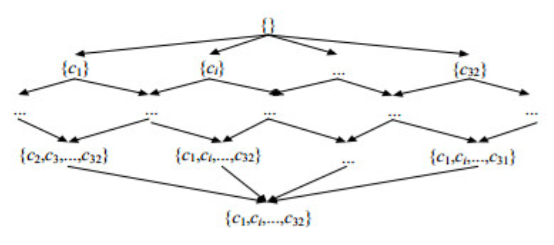
\includegraphics[scale=0.4]{Lattice.png}
  \caption{Lattice of taint propagation range.}
  \label{fig:Lattice}
\end{figure}
For any value x belongs to the value set V, the intersection operation $\cup$ takes the set combination set $\cup$, which includes: 

(1) x $ \wedge $ x = x, which satisfies the idempotency; 

(2) x $ \wedge $ y = y $ \wedge $ x, which satisfies the exchangeability;

(3) x $ \wedge $ (y $ \wedge $ z) = (x $ \wedge $ y) $ \wedge $z, which satisfies the Associativity. 

The top element is the empty set $\emptyset$, which is expressed as t, which has t$ \wedge $x = x for all x in V; the bottom element is the complete set u, which is expressed as $\perp$, which has $\perp\wedge$ x = $\perp$, for all x in V.

In the taint propagation logic, each statement stat corresponds to a transfer function FS, and the transfer function of a block containing multiple statements can be constructed by combining the transfer functions corresponding to each statement. The function set F is composed of a set of transfer functions $F_{S}$, whose input is the mapping $in[S]$ of the taint variable to the element in the lattice, and the input is a new mapping $out[S]$ after the taint propagation In forward taint propagation analysis, the transfer function $F_{S}$ takes $in[S]$ before the statement as the input and outputs $out[S]$ after the statement; the transfer function f is closed for combination operation, that is, for any function f and G in F, the function h with $H(x) = g(f(x))$ is also in F. there is a unit function I in the transfer function family F, which accepts a mapping as the same mapping returned by the input and output, that is, for All x in V, $I(x) = x$

Monotonicity is defined as: 

(1) for all F and X and Y in all V, $f (x \wedge  y) \leq f (x) \wedge f (y)$. 

Monotonicity can also be equivalently defined as: 

(2) for all F and X and Y in all V, $X \leq y$ implies $f (x) < f (y)$. It is proved that the two definitions are equivalent

It is proved that monotonicity(2) can be derived from monotonicity(1): since $x \wedge y$ is the maximum lower bound of X and y,$ X \wedge y \leq X$ and $X \wedge y \leq y$, from monotonicity(2), $f (x \wedge y) \leq f (x)$ and $f (x \wedge y) \leq f (y)$; at the same time, $f (x \wedge y)$ is the maximum lower bound of $f (x)$ and $f (y)$, monotonicity(1) is proved

Then, it is proved that monotonicity(1) can deduce monotonicity(2): suppose $x \leq y$, from monotonicity(1), $f (x \wedge y) \leq f (x) \wedge f (y)$, according to the definition, $x \wedge y = x$. therefore, $f (x) < f (x) \wedge f (y)$. Because $f (x \wedge y)$ is the maximum lower bound of $f (x)$ and $f (y)$, $f (x) \wedge f (y) < f (y)$, that is, $f (x) < f (y)$, monotonicity(2) is proved

The lattice\ref{fig:Lattice} shown clearly satisfies monotonicity (2) definite For any set X and Y, X belongs to $X \cup Y$.

\subsubsection{Taint sink}
The main choice of the taint slot is the exit function related to the network, and it can provide the log function. The log function is implemented by JNI.
\begin{figure}[ht]
  \centering
  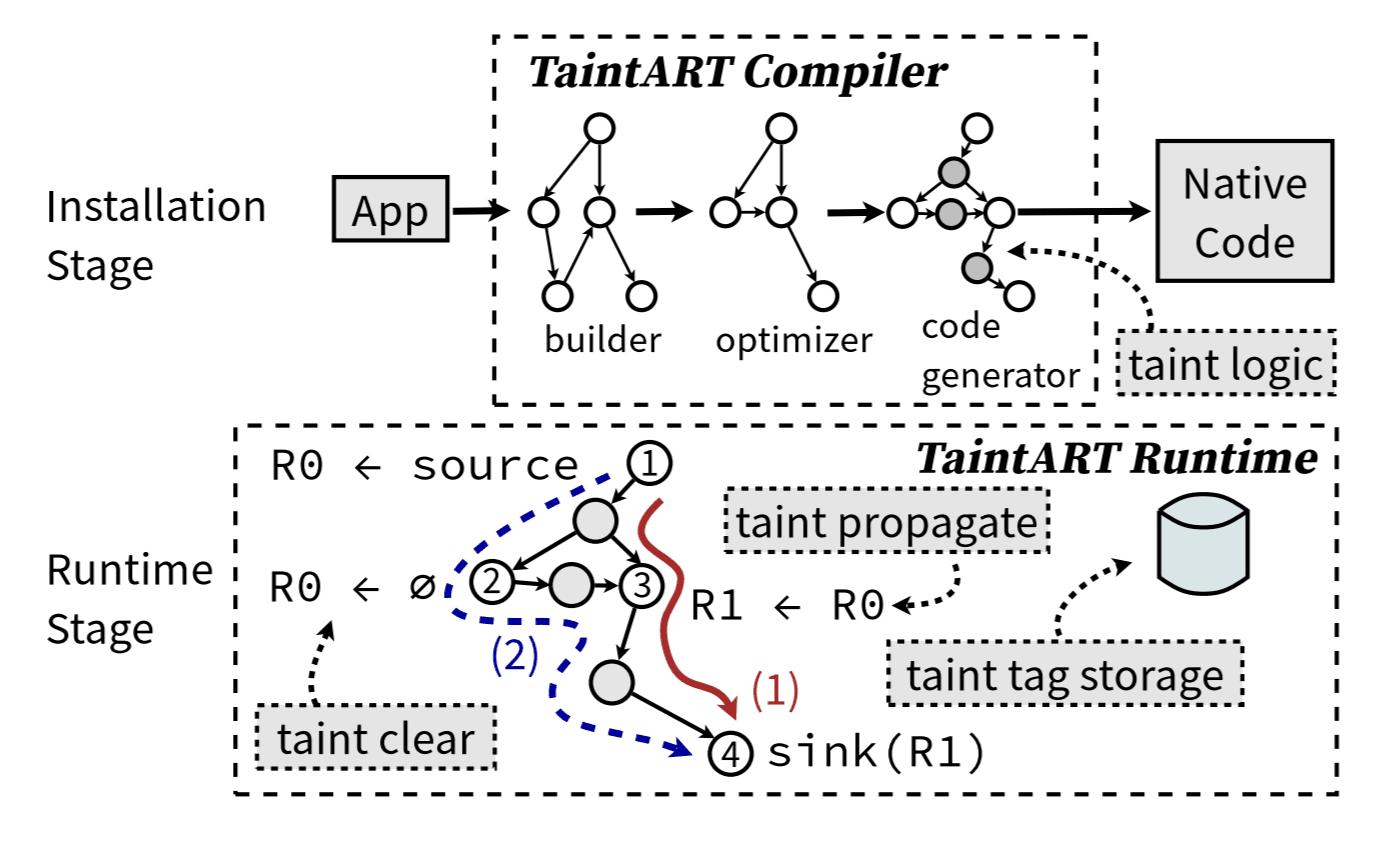
\includegraphics[scale=0.2]{TaintART4.png}
  \caption{Overview of TaintART.}
  \label{fig:TaintART4}
\end{figure}

\subsubsection{Taint tag storage}
Another feature of TaintART is its taint tag representation. Instead of the taint tag used by TaintDroid, the TaintART uses the concept of level. Figure \ref{fig:TaintART2} shows the table from TaintART. There are in total 4 levels where each of them consists some kind of data. Take level 2 as example. It represents both sensor data and location data. The system does not tell what exactly the information a variable carries. If a variable with level 2 information merge with a variable with level 1 information, the result will carry a level 2 tag. This is not desirable for the forensic purpose because of the need to tell the information flow as accurate as possible.

\begin{figure}[ht]
  \centering
  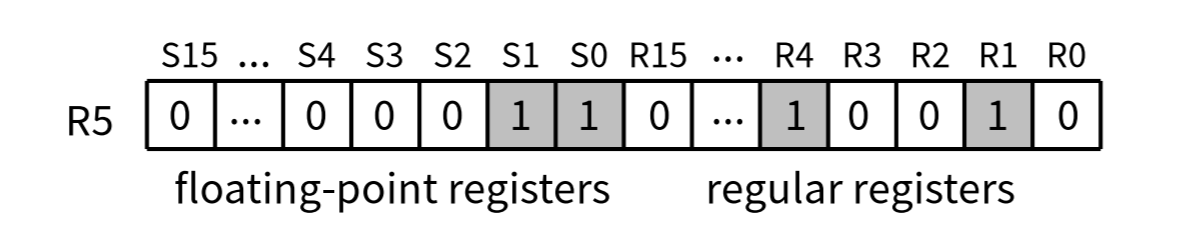
\includegraphics[scale=0.4]{TaintART5.png}
  \caption{Taint tag storage using Register R5.}
  \label{fig:TaintART5}
\end{figure}


\subsection{Principles of finding ICFG}
This part is completed through the FlowDroid, because only the FlowDroid can complete the control flow acquisition between components. In addition to the compiled APK, our input also includes the names of functions and tainted variables in DTA to reduce the number of branches that need to be optimized. This software simulates the full Android application life cycle to handle callbacks. Source and sink are detected by parsing the manifest file, art virtual machine bytecode file and XML layout file extracted from APK file. Finally, a dummy main function is generated to simulate the life cycle of activity, and a function call control flow chart (CFG) is established.

Because this software is based on soot, we can optimize it in the process of getting ICFG through soot, that is, if there are malicious function parts involved, we can replace or add wrappers.
\subsubsection{Definition of the lifecycle of android app}

FlowDroid generates a dummy main method that exactly mimics lifestyles.asynchronously executing component:An app may have multiple activities and services. FlowDroid assumes that all items can be executed asynchronously and analyzes the life cycle mentioned in the dummy main method. FlowDroid is path insensitive and does not need to consider all possible execution orders in the lifecycle.

When analyzing Android program to build call graph, we can't simply start from finding main method. All possible transfer relationships in the Android lifecycle must be modeled. The FlowDroid uses dummy main to simulate the life cycle. But the life cycle is not that simple. There are functions to save and restore state. Callback functions can also cause additional state changes.


\begin{figure}[ht]
  \centering
  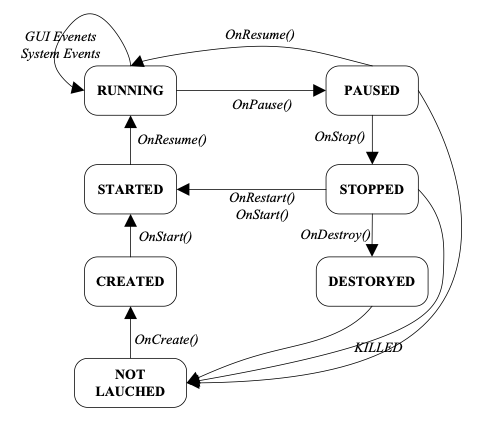
\includegraphics[scale=0.4]{FlowDroid1.png}
  \caption{the lifecycle of android app.}
  \label{fig:FlowDroid1}
\end{figure}


\begin{table}
  \caption{The functions in FlowDroid}
   \centering
   \begin{tabular}{ll}
     \toprule
       Function name  & Features \\
     \midrule
          
<de.ecspride.reflectionprivacyleak1.ReflectionPrivacyLeak1: void onStart()>& wrap leakage on start\\

<de.ecspride.reflectionprivacyleak1.ReflectionPrivacyLeak1: void onDestroy()> & wrap leakage on destroy\\

<de.ecspride.reflectionprivacyleak1.ReflectionPrivacyLeak1: void onPause()>& wrap leakage on pause\\

<de.ecspride.reflectionprivacyleak1.ReflectionPrivacyLeak1: void onRestart()>& wrap leakage on start\\

<de.ecspride.reflectionprivacyleak1.ReflectionPrivacyLeak1: void onResume()>& wrap leakage on resume\\

<de.ecspride.reflectionprivacyleak1.ReflectionPrivacyLeak1: void onStop()>& wrap leakage on stop\\

<de.ecspride.reflectionprivacyleak1.ReflectionPrivacyLeak1: void onCreate(android.os.Bundle)>&wrap leakage on create \\
     \bottomrule
   \end{tabular}
   
   \label{tab:table1}
 \end{table}

There are two ways to register callbacks,

(1)Register in XML: the XML file is mapped to multiple controls, the identifier is set, and the mapping is generated by tracking.

(2)Command mode: trace function call path in class file, generate function call control flow chart


\begin{figure}[ht]
  \centering
  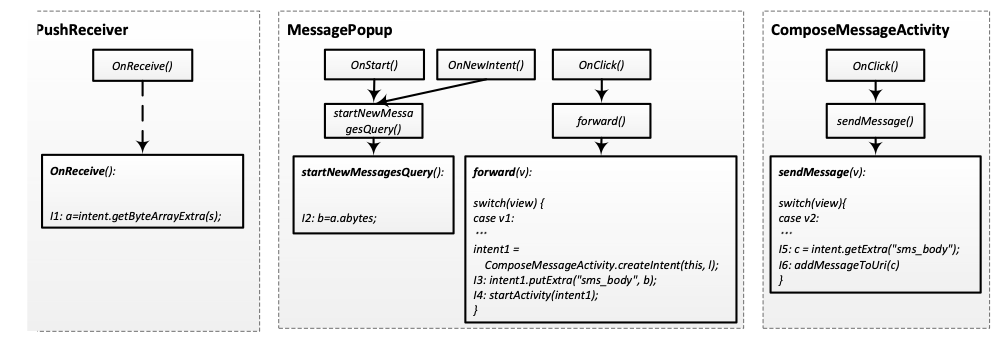
\includegraphics[scale=0.4]{FlowDroid4.png}
  \caption{the more detailed lifecycle of android app.}
  \label{fig:FlowDroid4}
\end{figure}

\subsubsection{Definition of the multiple entry point}

We define the entry point as the functions and variables output from the DTA, we can add the entry point by modifying $app.calculateSourcesSinksEntrypoints("SourcesAndSinks.txt");$

Through Flow droid, it'll treat those functions and variables as the dummy main and calculate the branch with them, and eventually output the related ICFG.

\subsubsection{Overview of the whole process}

Manifest.xml: apply global profile,

*.odex: Art virtual machine bytecode (application)

Layout XML layout profile

Android needs to extract the APK file first when running the program, then get the configuration information in the compiled Android manifest.xml file, and execute the ODEX program.

After decompressing the APK file, the functions related to the life cycle of FlowDroid, the callback functions, and the functions as source and sink.

The main method is then generated for the lifecycle and callback functions. The main method is used to generate call graph and inter procedural control flow graph (ICFG)

1) Unzipping APK file, which tracks the life cycle of activity and service by parsing XML, DEX and manifest files

2) FlowDroid generates dummy main method according to lifestyles and callback method, and establishes ICFG control flow chart

3) Report all flows from source to sink, including the information of the entire path

\begin{figure}[ht]
  \centering
  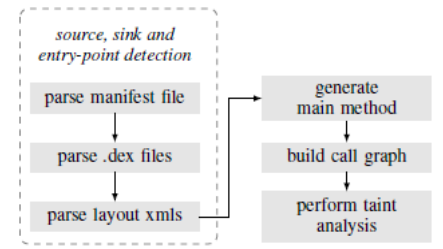
\includegraphics[scale=0.4]{FlowDroid3.png}
  \caption{TaintART Taint Propogation.}
  \label{fig:Overview of the whole process}
\end{figure}

\subsection{Principles of finding IFDS}
The analysis of data flow mainly depends on the Heros tools. It's hard to understand the relationship between Heros, Jasmin and soot at some time. Heros and jasmin are tools developed on the basis of soot, which are equivalent to the plug-ins of soot and can't run independently. Because there is no main call method of their own, the latest version of compiled soot.jar download contains these two tools by default.

Generally speaking, static stain analysis problems are all transformed into data flow analysis problems  for solution: first, build call graph (CG) according to the function call relationship in the program; second, in order to provide more fine-grained analysis of different execution paths of the program, also need to build control flow graph (CFG); finally, within and between processes, root According to different program characteristics, the specific data flow propagation analysis (and pointer analysis) is carried out. In the specific implementation, the stain analysis is often designed as an on-demand analysis algorithm: take the source function of the stain source as the driving source, analyze the propagation of its return value (stain) in the program until the sink function

IFDS framework  is an accurate and efficient framework for context sensitive and flow sensitive data flow analysis. It was proposed by reps et al. In 1996. The full name of IFDS is interprocedural, finite, distributive, subset problem. The problem works in a limited data basin, and the data flow fact needs to pass through the set of Union (or intersection) The operation satisfies the allocation rate. All the problems satisfying the above restrictions can be solved by IFDS algorithm (tabulation algorithm in reference ), and the problem of stain analysis just meets the requirements of IFDS problem. The data flow value of stain analysis is the stain variable, indicating that the current stain variable can reach the program point stmt. The worst time complexity of the algorithm is $O (ed^{3})$, in which e is the current control flow chart D is the size of the data basin.

The core idea of IFDSproblem solving algorithm is to transform program analysis problem into graph reachable problem . The analysis process of the algorithm is carried out on an expanded super graph (as shown in the example of Figure \ref{fig:IFDS}) constructed according to specific problems, in which data flow values can be shown as nodes in the graph. The algorithm extends a special data flow value: 0 value, which is used to represent empty sets; program analysis The calculation of the transfer function, that is, the transfer calculation of the data flow value, is transformed into the solution of the edge in the graph. In order to describe better, the algorithm decomposes the analysis into four kinds of transfer functions (edges) according to the characteristics of the program.

\begin{figure}[ht]
  \centering
  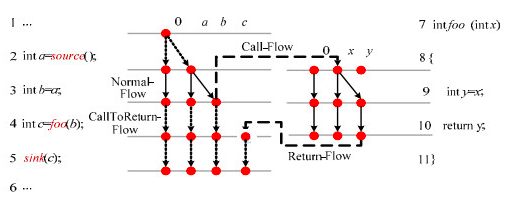
\includegraphics[scale=0.4]{IFDS.png}
  \caption{the process of IFDS.}
  \label{fig:IFDS}
\end{figure}
(1) Call flow is the transfer function to solve function call (parameter mapping)

(2) Return flow is the transfer function that solves the return value of function return statement to call point

(3) Calltoreturn flow is the transfer function from function call to function return

(4) Normal flow refers to the transfer function of statements other than the above three functions

IFDS algorithm tabulation is a dynamic programming algorithm, that is, the path of the solved subproblem can be reused. Because its data flow value meets the allocation rate, the edge can be merged in the branch or function call. The algorithm includes two kinds of path calculation: path edge and summary edge

the path edge represents the reachable path from the starting point to the current calculation point in the process

Abstract edge refers to the edge from function call to function return. Its main feature is that if the same function call is encountered again at different call points, its abstract edge information can be directly used to avoid repeated path edge calculation within the function

The following is an example in Figure \ref{fig:IFDS} to demonstrate how IFDS algorithm solves the problem of stain analysis. The data stream value represents the stain variable transmitted from the stain source. For simplicity, we abbreviate the stain source function as source (), and the leak point as sink (b), where B is the leak variable (the same below). As shown in line 2, an edge from 0 to a will be generated. For line 3, the assignment statement [b = a]; ]And a variable, normal flow is generally defined as: if the right value of the assignment statement is a stain variable, the left value is generated as a stain variable and the original value is retained, that is, the edge of a $\rightarrow$ B and a $\rightarrow$ A is generated. For the program function call in line 4, since B is the parameter of function foo, the analysis will start the call flow function. Call flow is generally defined as: if the argument is a stain variable, the stain of parameter will be generated correspondingly For the return point of the program function in line 10, return flow will generate the value of the return statement to the edge of the return value mapping of the call point, i.e. the edge of Y $\rightarrow$ C. for the sink function, if there is a data stream value passing through the statement, such as variable C in the figure, there is a path from 0 to statement sink (c), and C is the stain variable that finally triggers sink In foo, the calculated edge from the entrance to the exit (x $\rightarrow$ y in the figure) is analyzed and saved as the summary edge. After that, if foo is used in other locations of the program, the summary edge can be used directly

\section{Application Implementation}
\subsection{Useful Tools introduction}
\subsubsection{Soot}
Soot is a project with a long history. Its main purpose is to translate Java bytecode and DEX bytecode into an intermediate language. There are four ways to express the output results. Here, we mainly use jimple, which is very similar to Java. It uses less information to express the relationship between classes and variables. It can be described with only 15 opcodes.

Soot is the foundation of the whole static analysis framework. It can disassemble APK files. How to realize it in the middle doesn't need to be concerned for the time being. What the code finally gets is the middle representation. Through the API, you can access the members of each jimple, the call relationship, etc. according to this relationship, you can also generate a visible picture of CFG (control flow graph), which looks comfortable.

The documentation for \verb+Soot+ may be found at  \url{https://github.com/Sable/soot}
And the tutorial to optimize the android app's code listed here at \url{https://github.com/Sable/soot/wiki/Using-Soot-as-a-Program-Optimizer}. This part we didn't implement yet.
\subsection{Workflow}
We proposed to adapt the TaintART to automated DTA tools that we demands. \\

\begin{figure}[ht]
  \centering
  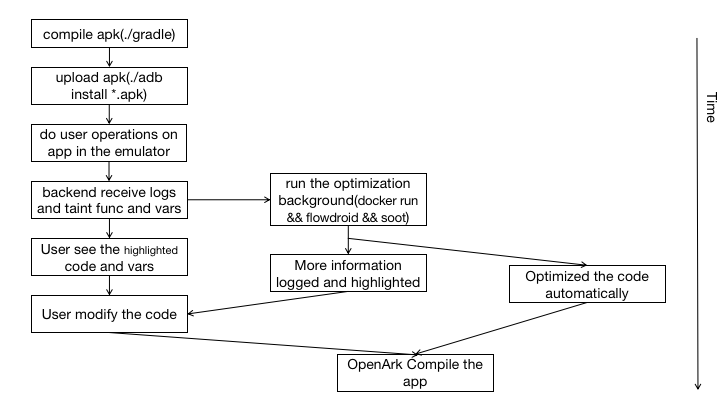
\includegraphics[scale=0.4]{ApakoHa.png}
  \caption{the process of ApakoHa.}
  \label{fig:ApakoHa}
\end{figure}

The source code is transferred to the qemu x86 64 virtual machine. Coverted to ART Runtime executable by dex2oat
                implemented with soot. In this step, TaintART performs a spot instrumentation operation. At runtime, TaintART uses the general-purpose register R5 to store the tags of the variables in the register, R1 to 3 passes the parameters between the methods, and R12 cooperates with the transfer of the internal operation of the register. A specific area is opened on the heap to store the taint information, so that the taint propagation logic can be detected To information leakage or potentially malicious behavior. After returning to the host, it will use soot(FlowDroid \& Heros) to perform static control flow analysis on the taint information and corresponding functions and APIs, and finally return it to the developer. The developer can modify the source code or use our auto optimization method to improve development efficiency. \\

\begin{figure}[ht]
  \centering
  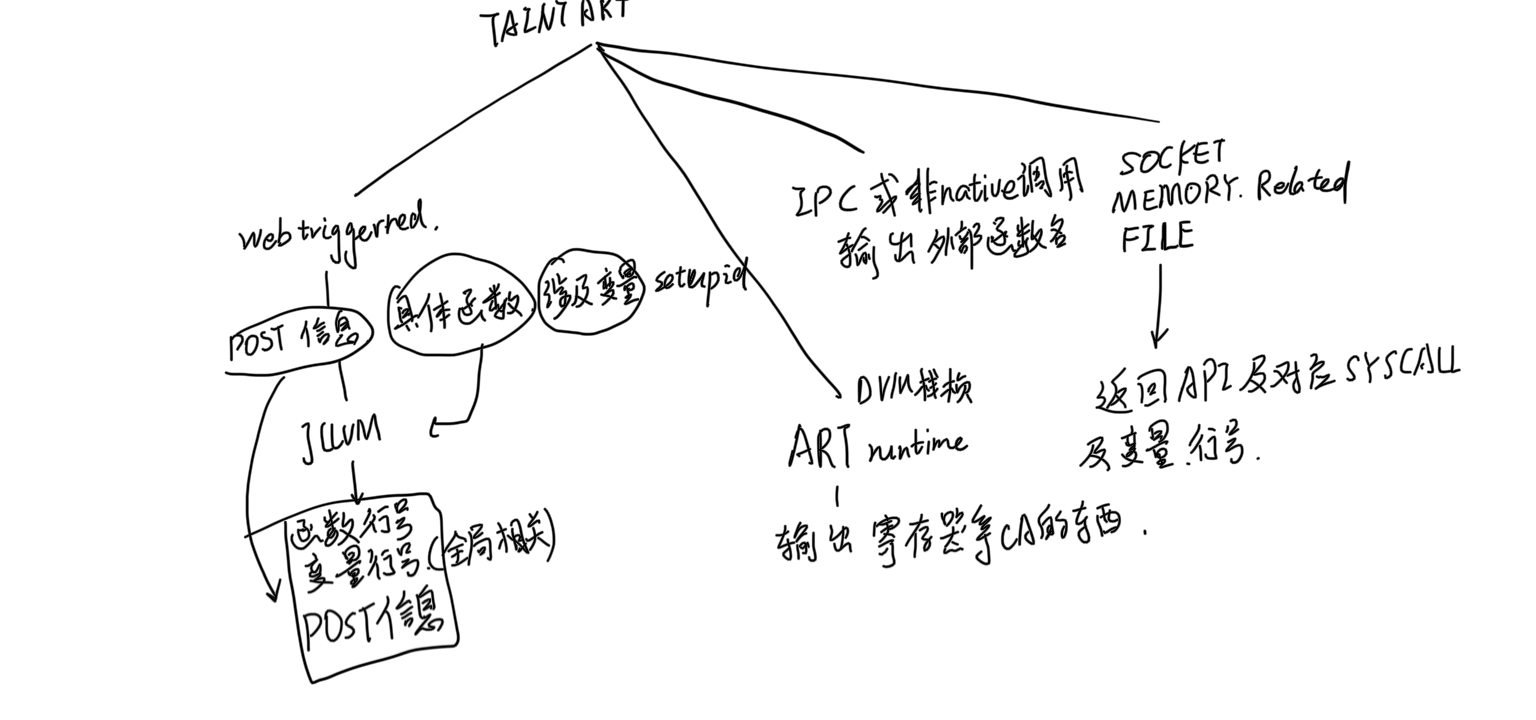
\includegraphics[scale=0.2]{2.png}
  \caption{the information of different source}
  \label{fig:2}
\end{figure}
As for the information of different source(like web, IPC, socket or memory and files), we adopt different methods to deal with.

\subsection{Display}

\begin{figure}[ht]
  \centering
  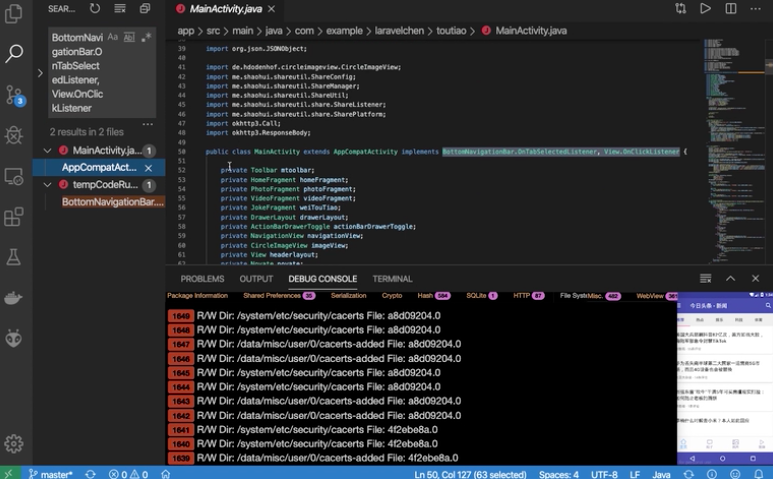
\includegraphics[scale=0.4]{Display1.png}
  \caption{the Display of \emph{ApakoHa}, DTA part}
  \label{fig:ApakoHa}
\end{figure}
\begin{figure}[ht]
  \centering
  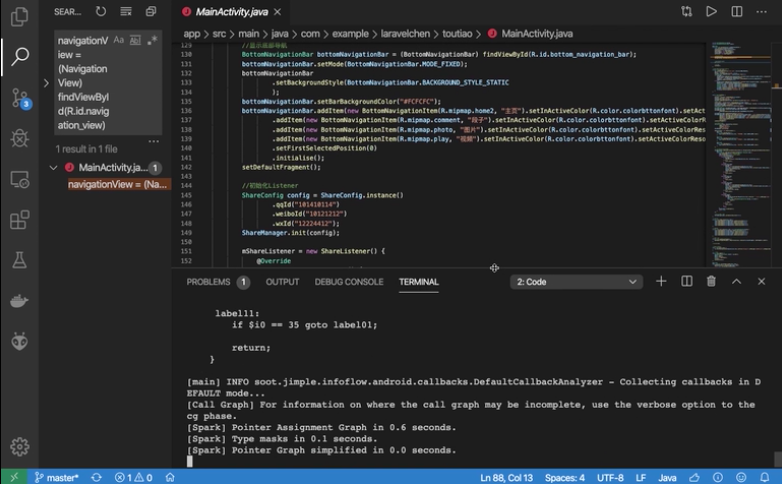
\includegraphics[scale=0.4]{Display2.png}
  \caption{the Display of \emph{ApakoHa}, STA oart}
  \label{fig:ApakoHa}
\end{figure}
\subsection{Benchmark}


\begin{table}
  \caption{The comparison of Control and Information analysis}
   \centering
   \begin{tabular}{lllll}
     \toprule
        & Control flow analysis &    & Information flow analysis& \\
     \midrule
      & mandatory access control  & Authority mechanism & STA & DTA\\
     High efficiency& low & middle  &  middle &  middle \\
     False positive rate& low &  low  & low  & high \\
     Missing report rate&  middle & middle   & low &low \\
     Flexibility& strong & strong &bad &bad \\
     Easiness of use& good &   middle&bad &bad \\
     \bottomrule
   \end{tabular}
   \label{tab:table1}
 \end{table}

 By using the information flow applying the DTA, the control flow's efficiency can be modified. In the process of optimization, those time will also be shortened.

 And here's the analyzing time, taking TouTiao as example.
 
 \begin{table}
  \caption{The comparison of the state of the art android taint analysis}
   \centering
   \begin{tabular}{lll}
     \toprule
       Name & Time & Note \\
     \midrule
      boot the virtual machine& <1s &just open and test\\
      test the app& 1min &should arrive branches as more as possible\\
      FlowDroid STA&20s &apply the control flow and information flow analysis\\
      soot optimization&unknown &not implemented\\
     \bottomrule
   \end{tabular}
   \label{tab:table1}
 \end{table}




\subsection{References}
  \begin{description}
    \item[\cite{Sun2016CCS}] A Practical Multi-level Information-Flow Tracking System for Android RunTime
    \item[\cite{ABDE2019WCNCW}] Android Malware Detection Based on System Calls Analysis and CNN Classification
    \item[\cite{Xu2018SPW}] A Dynamic Taint Analysis Tool for Android App Forensics
    \item[\cite{Yerima2014NGMAST}] Android Malware Detection Using Parallel Machine Learning Classifiers
    \item[\cite{Hsiao2014IMIS}] PasDroid: Real-Time Security Enhancement for Android
    \item[\cite{Ngu2017ICSE}] Cheetah: Just-in-Time Taint Analysis for Android Apps
    \item[\cite{Arzt2014SIGPLAN}]  FlowDroid: Precise Context, Flow, Field, Object-Sensitive and Lifecycle-Aware Taint Analysis for Android Apps
  \end{description}
  \label{sec:TaintDroid} 
  
% \end{thebibliography}


\end{document}
